\documentclass[twoside]{book}

% Packages required by doxygen
\usepackage{fixltx2e}
\usepackage{calc}
\usepackage{doxygen}
\usepackage[export]{adjustbox} % also loads graphicx
\usepackage{graphicx}
\usepackage[utf8]{inputenc}
\usepackage{makeidx}
\usepackage{multicol}
\usepackage{multirow}
\PassOptionsToPackage{warn}{textcomp}
\usepackage{textcomp}
\usepackage[nointegrals]{wasysym}
\usepackage[table]{xcolor}

% Font selection
\usepackage[T1]{fontenc}
\usepackage[scaled=.90]{helvet}
\usepackage{courier}
\usepackage{amssymb}
\usepackage{sectsty}
\renewcommand{\familydefault}{\sfdefault}
\allsectionsfont{%
  \fontseries{bc}\selectfont%
  \color{darkgray}%
}
\renewcommand{\DoxyLabelFont}{%
  \fontseries{bc}\selectfont%
  \color{darkgray}%
}
\newcommand{\+}{\discretionary{\mbox{\scriptsize$\hookleftarrow$}}{}{}}

% Page & text layout
\usepackage{geometry}
\geometry{%
  a4paper,%
  top=2.5cm,%
  bottom=2.5cm,%
  left=2.5cm,%
  right=2.5cm%
}
\tolerance=750
\hfuzz=15pt
\hbadness=750
\setlength{\emergencystretch}{15pt}
\setlength{\parindent}{0cm}
\setlength{\parskip}{3ex plus 2ex minus 2ex}
\makeatletter
\renewcommand{\paragraph}{%
  \@startsection{paragraph}{4}{0ex}{-1.0ex}{1.0ex}{%
    \normalfont\normalsize\bfseries\SS@parafont%
  }%
}
\renewcommand{\subparagraph}{%
  \@startsection{subparagraph}{5}{0ex}{-1.0ex}{1.0ex}{%
    \normalfont\normalsize\bfseries\SS@subparafont%
  }%
}
\makeatother

% Headers & footers
\usepackage{fancyhdr}
\pagestyle{fancyplain}
\fancyhead[LE]{\fancyplain{}{\bfseries\thepage}}
\fancyhead[CE]{\fancyplain{}{}}
\fancyhead[RE]{\fancyplain{}{\bfseries\leftmark}}
\fancyhead[LO]{\fancyplain{}{\bfseries\rightmark}}
\fancyhead[CO]{\fancyplain{}{}}
\fancyhead[RO]{\fancyplain{}{\bfseries\thepage}}
\fancyfoot[LE]{\fancyplain{}{}}
\fancyfoot[CE]{\fancyplain{}{}}
\fancyfoot[RE]{\fancyplain{}{\bfseries\scriptsize Generated by Doxygen }}
\fancyfoot[LO]{\fancyplain{}{\bfseries\scriptsize Generated by Doxygen }}
\fancyfoot[CO]{\fancyplain{}{}}
\fancyfoot[RO]{\fancyplain{}{}}
\renewcommand{\footrulewidth}{0.4pt}
\renewcommand{\chaptermark}[1]{%
  \markboth{#1}{}%
}
\renewcommand{\sectionmark}[1]{%
  \markright{\thesection\ #1}%
}

% Indices & bibliography
\usepackage{natbib}
\usepackage[titles]{tocloft}
\setcounter{tocdepth}{3}
\setcounter{secnumdepth}{5}
\makeindex

% Hyperlinks (required, but should be loaded last)
\usepackage{ifpdf}
\ifpdf
  \usepackage[pdftex,pagebackref=true]{hyperref}
\else
  \usepackage[ps2pdf,pagebackref=true]{hyperref}
\fi
\hypersetup{%
  colorlinks=true,%
  linkcolor=blue,%
  citecolor=blue,%
  unicode%
}

% Custom commands
\newcommand{\clearemptydoublepage}{%
  \newpage{\pagestyle{empty}\cleardoublepage}%
}

\usepackage{caption}
\captionsetup{labelsep=space,justification=centering,font={bf},singlelinecheck=off,skip=4pt,position=top}

%===== C O N T E N T S =====

\begin{document}

% Titlepage & ToC
\hypersetup{pageanchor=false,
             bookmarksnumbered=true,
             pdfencoding=unicode
            }
\pagenumbering{alph}
\begin{titlepage}
\vspace*{7cm}
\begin{center}%
{\Large Heislab Eirik og Henrik }\\
\vspace*{1cm}
{\large Generated by Doxygen 1.8.13}\\
\end{center}
\end{titlepage}
\clearemptydoublepage
\pagenumbering{roman}
\tableofcontents
\clearemptydoublepage
\pagenumbering{arabic}
\hypersetup{pageanchor=true}

%--- Begin generated contents ---
\chapter{File Index}
\section{File List}
Here is a list of all documented files with brief descriptions\+:\begin{DoxyCompactList}
\item\contentsline{section}{source/\hyperlink{fsm_8c}{fsm.\+c} \\*.c-\/file for setting up the elevators finite state machine (fsm) }{\pageref{fsm_8c}}{}
\item\contentsline{section}{source/\hyperlink{fsm_8h}{fsm.\+h} \\*.h-\/file for setting up the elevators finite state machine (fsm) }{\pageref{fsm_8h}}{}
\item\contentsline{section}{source/\hyperlink{main_8c}{main.\+c} \\*Main file }{\pageref{main_8c}}{}
\item\contentsline{section}{source/\hyperlink{queue_8c}{queue.\+c} \\*.c-\/file that contains all the logic for queue management in the elevator queue }{\pageref{queue_8c}}{}
\item\contentsline{section}{source/\hyperlink{queue_8h}{queue.\+h} \\*.h-\/file for handling orders and managing the elevator queue }{\pageref{queue_8h}}{}
\item\contentsline{section}{source/\hyperlink{timer_8c}{timer.\+c} \\*.c-\/file for the timer system }{\pageref{timer_8c}}{}
\item\contentsline{section}{source/\hyperlink{timer_8h}{timer.\+h} \\*.h-\/file for the timer system }{\pageref{timer_8h}}{}
\end{DoxyCompactList}

\chapter{File Documentation}
\hypertarget{fsm_8c}{}\section{source/fsm.c File Reference}
\label{fsm_8c}\index{source/fsm.\+c@{source/fsm.\+c}}


.c-\/file for setting up the elevators finite state machine (fsm)  


{\ttfamily \#include \char`\"{}fsm.\+h\char`\"{}}\newline
{\ttfamily \#include $<$stdio.\+h$>$}\newline
{\ttfamily \#include $<$stdlib.\+h$>$}\newline
Include dependency graph for fsm.\+c\+:
\nopagebreak
\begin{figure}[H]
\begin{center}
\leavevmode
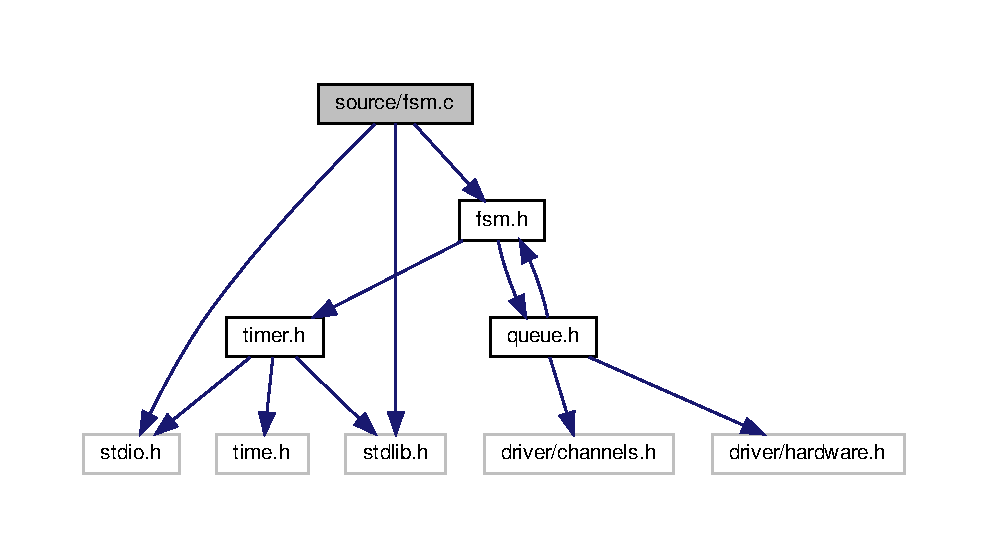
\includegraphics[width=350pt]{fsm_8c__incl}
\end{center}
\end{figure}
\subsection*{Functions}
\begin{DoxyCompactItemize}
\item 
\mbox{\Hypertarget{fsm_8c_a8ee1eda139065a11895e51ca67038ac9}\label{fsm_8c_a8ee1eda139065a11895e51ca67038ac9}} 
void \hyperlink{fsm_8c_a8ee1eda139065a11895e51ca67038ac9}{fsm\+\_\+update\+\_\+elevator\+\_\+position\+\_\+at\+\_\+floor} ()
\begin{DoxyCompactList}\small\item\em Updates the position of the elevator when the elevator arrives at a new floor. \end{DoxyCompactList}\item 
int \hyperlink{fsm_8c_a573c28869d86e2ee8eb3f7a28a7054e3}{fsm\+\_\+elevator\+\_\+is\+\_\+at\+\_\+floor} ()
\begin{DoxyCompactList}\small\item\em Checks if the elevator receives a floor sensor signal/if the elevator is at a floor. \end{DoxyCompactList}\item 
\mbox{\Hypertarget{fsm_8c_ace237751f33298751285a2a4a5c60d1d}\label{fsm_8c_ace237751f33298751285a2a4a5c60d1d}} 
void \hyperlink{fsm_8c_ace237751f33298751285a2a4a5c60d1d}{fsm\+\_\+update\+\_\+elevator\+\_\+position\+\_\+between\+\_\+floors} ()
\begin{DoxyCompactList}\small\item\em Updates the position of the elevator when the elevator is between two floors. \end{DoxyCompactList}\item 
int \hyperlink{fsm_8c_a97ef7bccac097b8a3f00b84aa346243e}{fsm\+\_\+stop\+\_\+elevator\+\_\+at\+\_\+floor} ()
\begin{DoxyCompactList}\small\item\em Checks orders, elevator position and direction, and decides whether to stop or not at the floor the elevator is passing by. \end{DoxyCompactList}\item 
\mbox{\Hypertarget{fsm_8c_abfbebabfd006bb1ad394c58906a5ebb4}\label{fsm_8c_abfbebabfd006bb1ad394c58906a5ebb4}} 
void \hyperlink{fsm_8c_abfbebabfd006bb1ad394c58906a5ebb4}{fsm\+\_\+choose\+\_\+motor\+\_\+direction} ()
\begin{DoxyCompactList}\small\item\em Checks orders, elevator position and direction, and chooses motordirection up/down when the elevator goes from still to moving. \end{DoxyCompactList}\item 
\mbox{\Hypertarget{fsm_8c_a05121e3cfc372d76f6052c0d4c032090}\label{fsm_8c_a05121e3cfc372d76f6052c0d4c032090}} 
void \hyperlink{fsm_8c_a05121e3cfc372d76f6052c0d4c032090}{fsm\+\_\+state\+\_\+machine} ()
\begin{DoxyCompactList}\small\item\em The finite state machine switch-\/case function. Sets and changes the elevator state. \end{DoxyCompactList}\end{DoxyCompactItemize}
\subsection*{Variables}
\begin{DoxyCompactItemize}
\item 
\mbox{\Hypertarget{fsm_8c_ac1f47f38d29870d6d5908c517eda6475}\label{fsm_8c_ac1f47f38d29870d6d5908c517eda6475}} 
\hyperlink{fsm_8h_acd367487f07fca9e254fc824e3e611a8}{elevator\+\_\+state} \hyperlink{fsm_8c_ac1f47f38d29870d6d5908c517eda6475}{now\+\_\+state} = I\+N\+IT
\begin{DoxyCompactList}\small\item\em Variable for storing the current state of the elevator. \end{DoxyCompactList}\item 
\mbox{\Hypertarget{fsm_8c_ab1cb5a3b17a40ee0f3ca79db5625b740}\label{fsm_8c_ab1cb5a3b17a40ee0f3ca79db5625b740}} 
Hardware\+Movement \hyperlink{fsm_8c_ab1cb5a3b17a40ee0f3ca79db5625b740}{previous\+\_\+direction} = H\+A\+R\+D\+W\+A\+R\+E\+\_\+\+M\+O\+V\+E\+M\+E\+N\+T\+\_\+\+D\+O\+WN
\begin{DoxyCompactList}\small\item\em Variable for storing the previous direction the elevator was moving in. \end{DoxyCompactList}\item 
\mbox{\Hypertarget{fsm_8c_a1046f1be4602c42ef4fe8de2ed351c66}\label{fsm_8c_a1046f1be4602c42ef4fe8de2ed351c66}} 
Hardware\+Movement \hyperlink{fsm_8c_a1046f1be4602c42ef4fe8de2ed351c66}{current\+\_\+direction} = H\+A\+R\+D\+W\+A\+R\+E\+\_\+\+M\+O\+V\+E\+M\+E\+N\+T\+\_\+\+D\+O\+WN
\begin{DoxyCompactList}\small\item\em Variable for storing the direction the elevator is currently moving in. \end{DoxyCompactList}\end{DoxyCompactItemize}


\subsection{Detailed Description}
.c-\/file for setting up the elevators finite state machine (fsm) 



\subsection{Function Documentation}
\mbox{\Hypertarget{fsm_8c_a573c28869d86e2ee8eb3f7a28a7054e3}\label{fsm_8c_a573c28869d86e2ee8eb3f7a28a7054e3}} 
\index{fsm.\+c@{fsm.\+c}!fsm\+\_\+elevator\+\_\+is\+\_\+at\+\_\+floor@{fsm\+\_\+elevator\+\_\+is\+\_\+at\+\_\+floor}}
\index{fsm\+\_\+elevator\+\_\+is\+\_\+at\+\_\+floor@{fsm\+\_\+elevator\+\_\+is\+\_\+at\+\_\+floor}!fsm.\+c@{fsm.\+c}}
\subsubsection{\texorpdfstring{fsm\+\_\+elevator\+\_\+is\+\_\+at\+\_\+floor()}{fsm\_elevator\_is\_at\_floor()}}
{\footnotesize\ttfamily int fsm\+\_\+elevator\+\_\+is\+\_\+at\+\_\+floor (\begin{DoxyParamCaption}{ }\end{DoxyParamCaption})}



Checks if the elevator receives a floor sensor signal/if the elevator is at a floor. 

\begin{DoxyReturn}{Returns}
1 If the elevator is at a floor. 

0 If the elevator is between two floors/not at a floor. 
\end{DoxyReturn}


Definition at line 25 of file fsm.\+c.

\mbox{\Hypertarget{fsm_8c_a97ef7bccac097b8a3f00b84aa346243e}\label{fsm_8c_a97ef7bccac097b8a3f00b84aa346243e}} 
\index{fsm.\+c@{fsm.\+c}!fsm\+\_\+stop\+\_\+elevator\+\_\+at\+\_\+floor@{fsm\+\_\+stop\+\_\+elevator\+\_\+at\+\_\+floor}}
\index{fsm\+\_\+stop\+\_\+elevator\+\_\+at\+\_\+floor@{fsm\+\_\+stop\+\_\+elevator\+\_\+at\+\_\+floor}!fsm.\+c@{fsm.\+c}}
\subsubsection{\texorpdfstring{fsm\+\_\+stop\+\_\+elevator\+\_\+at\+\_\+floor()}{fsm\_stop\_elevator\_at\_floor()}}
{\footnotesize\ttfamily int fsm\+\_\+stop\+\_\+elevator\+\_\+at\+\_\+floor (\begin{DoxyParamCaption}{ }\end{DoxyParamCaption})}



Checks orders, elevator position and direction, and decides whether to stop or not at the floor the elevator is passing by. 

\begin{DoxyReturn}{Returns}
1 If the elevator should stop. 

0 If the elevator should keep moving. 
\end{DoxyReturn}


Definition at line 54 of file fsm.\+c.


\hypertarget{fsm_8h}{}\section{source/fsm.h File Reference}
\label{fsm_8h}\index{source/fsm.\+h@{source/fsm.\+h}}


.h-\/file for setting up the elevators finite state machine (fsm).  


{\ttfamily \#include \char`\"{}queue.\+h\char`\"{}}\newline
{\ttfamily \#include \char`\"{}timer.\+h\char`\"{}}\newline
Include dependency graph for fsm.\+h\+:
\nopagebreak
\begin{figure}[H]
\begin{center}
\leavevmode
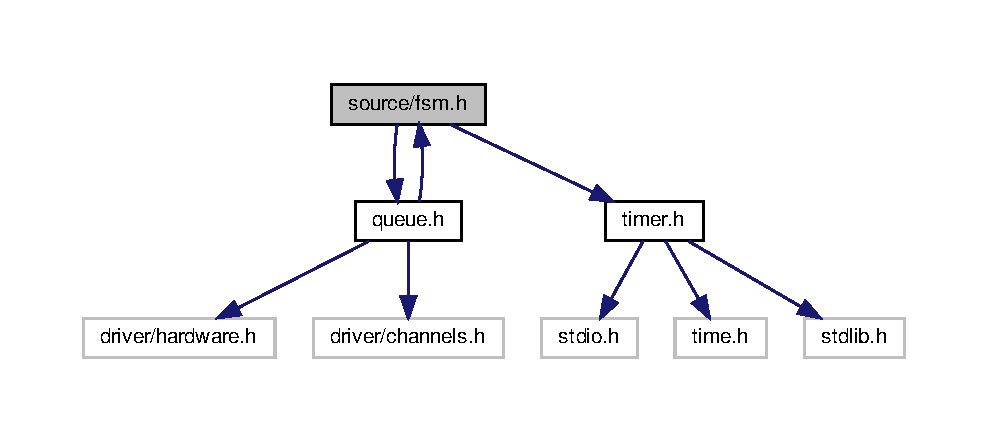
\includegraphics[width=350pt]{fsm_8h__incl}
\end{center}
\end{figure}
This graph shows which files directly or indirectly include this file\+:
\nopagebreak
\begin{figure}[H]
\begin{center}
\leavevmode
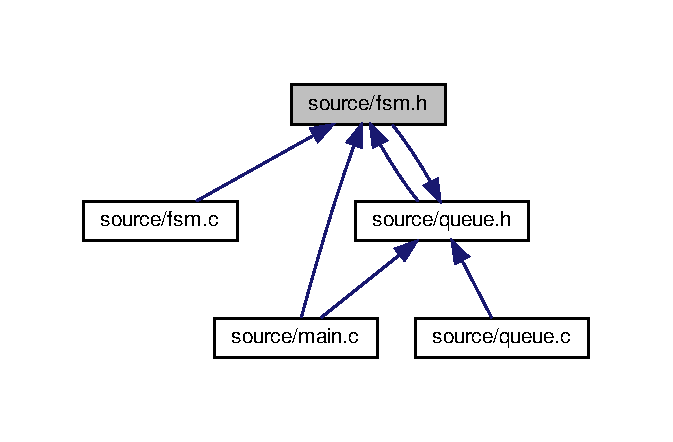
\includegraphics[width=323pt]{fsm_8h__dep__incl}
\end{center}
\end{figure}
\subsection*{Enumerations}
\begin{DoxyCompactItemize}
\item 
\mbox{\Hypertarget{fsm_8h_acd367487f07fca9e254fc824e3e611a8}\label{fsm_8h_acd367487f07fca9e254fc824e3e611a8}} 
enum \hyperlink{fsm_8h_acd367487f07fca9e254fc824e3e611a8}{elevator\+\_\+state} \{ \newline
{\bfseries I\+N\+IT}, 
{\bfseries I\+D\+LE}, 
{\bfseries M\+O\+V\+I\+NG}, 
{\bfseries O\+P\+E\+N\+\_\+\+D\+O\+OR}, 
\newline
{\bfseries S\+T\+O\+P\+\_\+\+B\+E\+T\+W\+E\+E\+N\+\_\+\+F\+L\+O\+O\+RS}, 
{\bfseries S\+T\+O\+P\+\_\+\+A\+T\+\_\+\+F\+L\+O\+OR}
 \}\begin{DoxyCompactList}\small\item\em Enum containing the different states of the elevator in the fsm. \end{DoxyCompactList}
\end{DoxyCompactItemize}
\subsection*{Functions}
\begin{DoxyCompactItemize}
\item 
int \hyperlink{fsm_8h_a573c28869d86e2ee8eb3f7a28a7054e3}{fsm\+\_\+elevator\+\_\+is\+\_\+at\+\_\+floor} ()
\begin{DoxyCompactList}\small\item\em Checks if the elevator receives a floor sensor signal/if the elevator is at a floor. \end{DoxyCompactList}\item 
\mbox{\Hypertarget{fsm_8h_a8ee1eda139065a11895e51ca67038ac9}\label{fsm_8h_a8ee1eda139065a11895e51ca67038ac9}} 
void \hyperlink{fsm_8h_a8ee1eda139065a11895e51ca67038ac9}{fsm\+\_\+update\+\_\+elevator\+\_\+position\+\_\+at\+\_\+floor} ()
\begin{DoxyCompactList}\small\item\em Updates the position of the elevator when the elevator arrives at a new floor. \end{DoxyCompactList}\item 
\mbox{\Hypertarget{fsm_8h_ace237751f33298751285a2a4a5c60d1d}\label{fsm_8h_ace237751f33298751285a2a4a5c60d1d}} 
void \hyperlink{fsm_8h_ace237751f33298751285a2a4a5c60d1d}{fsm\+\_\+update\+\_\+elevator\+\_\+position\+\_\+between\+\_\+floors} ()
\begin{DoxyCompactList}\small\item\em Updates the position of the elevator when the elevator is between two floors. \end{DoxyCompactList}\item 
int \hyperlink{fsm_8h_a97ef7bccac097b8a3f00b84aa346243e}{fsm\+\_\+stop\+\_\+elevator\+\_\+at\+\_\+floor} ()
\begin{DoxyCompactList}\small\item\em Checks orders, elevator position and direction, and decides whether to stop or not at the floor the elevator is passing by. \end{DoxyCompactList}\item 
\mbox{\Hypertarget{fsm_8h_abfbebabfd006bb1ad394c58906a5ebb4}\label{fsm_8h_abfbebabfd006bb1ad394c58906a5ebb4}} 
void \hyperlink{fsm_8h_abfbebabfd006bb1ad394c58906a5ebb4}{fsm\+\_\+choose\+\_\+motor\+\_\+direction} ()
\begin{DoxyCompactList}\small\item\em Checks orders, elevator position and direction, and chooses motordirection up/down when the elevator goes from still to moving. \end{DoxyCompactList}\item 
\mbox{\Hypertarget{fsm_8h_a05121e3cfc372d76f6052c0d4c032090}\label{fsm_8h_a05121e3cfc372d76f6052c0d4c032090}} 
void \hyperlink{fsm_8h_a05121e3cfc372d76f6052c0d4c032090}{fsm\+\_\+state\+\_\+machine} ()
\begin{DoxyCompactList}\small\item\em The finite state machine switch-\/case function. Sets and changes the elevator state. \end{DoxyCompactList}\end{DoxyCompactItemize}
\subsection*{Variables}
\begin{DoxyCompactItemize}
\item 
\mbox{\Hypertarget{fsm_8h_ac1f47f38d29870d6d5908c517eda6475}\label{fsm_8h_ac1f47f38d29870d6d5908c517eda6475}} 
\hyperlink{fsm_8h_acd367487f07fca9e254fc824e3e611a8}{elevator\+\_\+state} \hyperlink{fsm_8h_ac1f47f38d29870d6d5908c517eda6475}{now\+\_\+state}
\begin{DoxyCompactList}\small\item\em Variable for storing the current state of the elevator. \end{DoxyCompactList}\item 
\mbox{\Hypertarget{fsm_8h_ab1cb5a3b17a40ee0f3ca79db5625b740}\label{fsm_8h_ab1cb5a3b17a40ee0f3ca79db5625b740}} 
Hardware\+Movement \hyperlink{fsm_8h_ab1cb5a3b17a40ee0f3ca79db5625b740}{previous\+\_\+direction}
\begin{DoxyCompactList}\small\item\em Variable for storing the previous direction the elevator was moving in. \end{DoxyCompactList}\item 
\mbox{\Hypertarget{fsm_8h_a1046f1be4602c42ef4fe8de2ed351c66}\label{fsm_8h_a1046f1be4602c42ef4fe8de2ed351c66}} 
Hardware\+Movement \hyperlink{fsm_8h_a1046f1be4602c42ef4fe8de2ed351c66}{current\+\_\+direction}
\begin{DoxyCompactList}\small\item\em Variable for storing the direction the elevator is currently moving in. \end{DoxyCompactList}\end{DoxyCompactItemize}


\subsection{Detailed Description}
.h-\/file for setting up the elevators finite state machine (fsm). 



\subsection{Function Documentation}
\mbox{\Hypertarget{fsm_8h_a573c28869d86e2ee8eb3f7a28a7054e3}\label{fsm_8h_a573c28869d86e2ee8eb3f7a28a7054e3}} 
\index{fsm.\+h@{fsm.\+h}!fsm\+\_\+elevator\+\_\+is\+\_\+at\+\_\+floor@{fsm\+\_\+elevator\+\_\+is\+\_\+at\+\_\+floor}}
\index{fsm\+\_\+elevator\+\_\+is\+\_\+at\+\_\+floor@{fsm\+\_\+elevator\+\_\+is\+\_\+at\+\_\+floor}!fsm.\+h@{fsm.\+h}}
\subsubsection{\texorpdfstring{fsm\+\_\+elevator\+\_\+is\+\_\+at\+\_\+floor()}{fsm\_elevator\_is\_at\_floor()}}
{\footnotesize\ttfamily int fsm\+\_\+elevator\+\_\+is\+\_\+at\+\_\+floor (\begin{DoxyParamCaption}{ }\end{DoxyParamCaption})}



Checks if the elevator receives a floor sensor signal/if the elevator is at a floor. 

\begin{DoxyReturn}{Returns}
1 If the elevator is at a floor. 

0 If the elevator is between two floors/not at a floor. 
\end{DoxyReturn}


Definition at line 25 of file fsm.\+c.

\mbox{\Hypertarget{fsm_8h_a97ef7bccac097b8a3f00b84aa346243e}\label{fsm_8h_a97ef7bccac097b8a3f00b84aa346243e}} 
\index{fsm.\+h@{fsm.\+h}!fsm\+\_\+stop\+\_\+elevator\+\_\+at\+\_\+floor@{fsm\+\_\+stop\+\_\+elevator\+\_\+at\+\_\+floor}}
\index{fsm\+\_\+stop\+\_\+elevator\+\_\+at\+\_\+floor@{fsm\+\_\+stop\+\_\+elevator\+\_\+at\+\_\+floor}!fsm.\+h@{fsm.\+h}}
\subsubsection{\texorpdfstring{fsm\+\_\+stop\+\_\+elevator\+\_\+at\+\_\+floor()}{fsm\_stop\_elevator\_at\_floor()}}
{\footnotesize\ttfamily int fsm\+\_\+stop\+\_\+elevator\+\_\+at\+\_\+floor (\begin{DoxyParamCaption}{ }\end{DoxyParamCaption})}



Checks orders, elevator position and direction, and decides whether to stop or not at the floor the elevator is passing by. 

\begin{DoxyReturn}{Returns}
1 If the elevator should stop. 

0 If the elevator should keep moving. 
\end{DoxyReturn}


Definition at line 54 of file fsm.\+c.


\hypertarget{main_8c}{}\section{source/main.c File Reference}
\label{main_8c}\index{source/main.\+c@{source/main.\+c}}


Main file.  


{\ttfamily \#include $<$stdio.\+h$>$}\newline
{\ttfamily \#include $<$stdlib.\+h$>$}\newline
{\ttfamily \#include $<$signal.\+h$>$}\newline
{\ttfamily \#include \char`\"{}driver/hardware.\+h\char`\"{}}\newline
{\ttfamily \#include \char`\"{}queue.\+h\char`\"{}}\newline
{\ttfamily \#include \char`\"{}fsm.\+h\char`\"{}}\newline
Include dependency graph for main.\+c\+:
\nopagebreak
\begin{figure}[H]
\begin{center}
\leavevmode
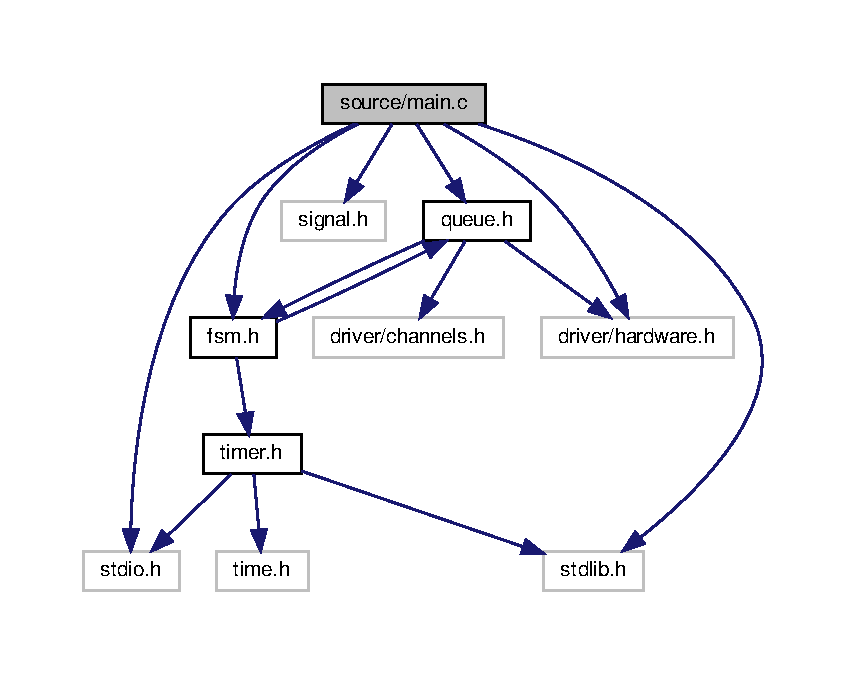
\includegraphics[width=350pt]{main_8c__incl}
\end{center}
\end{figure}
\subsection*{Functions}
\begin{DoxyCompactItemize}
\item 
\mbox{\Hypertarget{main_8c_ae66f6b31b5ad750f1fe042a706a4e3d4}\label{main_8c_ae66f6b31b5ad750f1fe042a706a4e3d4}} 
int \hyperlink{main_8c_ae66f6b31b5ad750f1fe042a706a4e3d4}{main} ()
\begin{DoxyCompactList}\small\item\em Main function of the program. Runs the state machine. \end{DoxyCompactList}\end{DoxyCompactItemize}


\subsection{Detailed Description}
Main file. 


\hypertarget{queue_8c}{}\section{source/queue.c File Reference}
\label{queue_8c}\index{source/queue.\+c@{source/queue.\+c}}


.c-\/file that contains all the logic for queue management in the elevator queue.  


{\ttfamily \#include \char`\"{}queue.\+h\char`\"{}}\newline
{\ttfamily \#include $<$stdio.\+h$>$}\newline
{\ttfamily \#include $<$stdlib.\+h$>$}\newline
Include dependency graph for queue.\+c\+:
\nopagebreak
\begin{figure}[H]
\begin{center}
\leavevmode
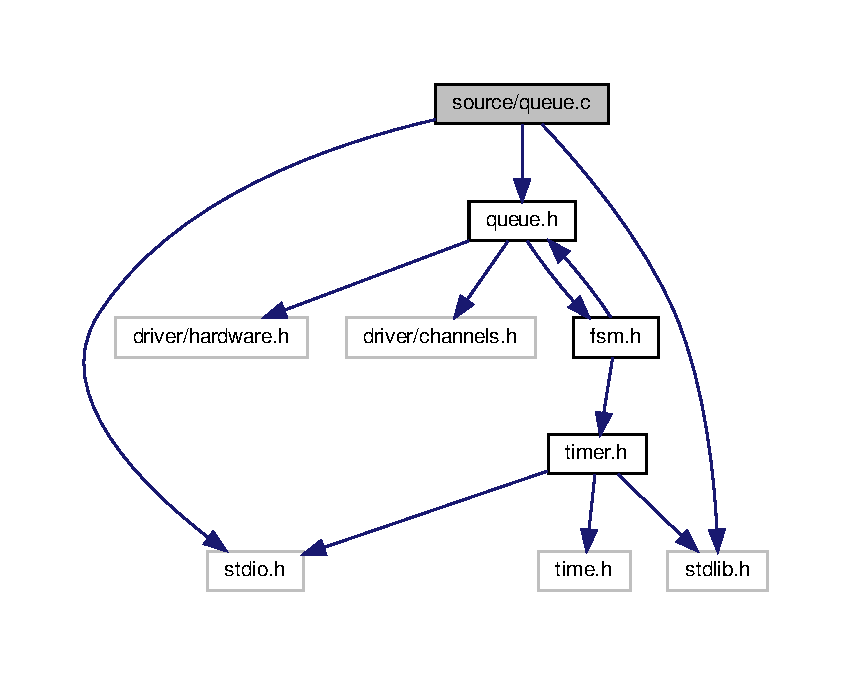
\includegraphics[width=350pt]{queue_8c__incl}
\end{center}
\end{figure}
\subsection*{Functions}
\begin{DoxyCompactItemize}
\item 
\mbox{\Hypertarget{queue_8c_a9d79c1ab7ae2f8d03fa045eae25f6b2a}\label{queue_8c_a9d79c1ab7ae2f8d03fa045eae25f6b2a}} 
void \hyperlink{queue_8c_a9d79c1ab7ae2f8d03fa045eae25f6b2a}{queue\+\_\+init\+\_\+queue} ()
\begin{DoxyCompactList}\small\item\em Initializes the queue matrix. \end{DoxyCompactList}\item 
int \hyperlink{queue_8c_af2004759a602f00d51d7a52b842ee27e}{queue\+\_\+queue\+\_\+exists} ()
\begin{DoxyCompactList}\small\item\em Checks if the queue contains order(s). \end{DoxyCompactList}\item 
\mbox{\Hypertarget{queue_8c_a3e5f178d15a689153f9d101a5e15b905}\label{queue_8c_a3e5f178d15a689153f9d101a5e15b905}} 
void \hyperlink{queue_8c_a3e5f178d15a689153f9d101a5e15b905}{queue\+\_\+iterate\+\_\+and\+\_\+update\+\_\+queue} ()
\begin{DoxyCompactList}\small\item\em Checks the hardware for orders and inserts them in the queue. Sets order-\/lights in hardware. \end{DoxyCompactList}\item 
int \hyperlink{queue_8c_a66cc5e1def51a8612fe8b6299c629ec3}{queue\+\_\+order\+\_\+above\+\_\+current\+\_\+position} (\hyperlink{queue_8h_a3f7930823335655eba2f898c739671d0}{elevator\+\_\+position} \hyperlink{queue_8h_a64aa88f4f8e0b2dc9d03a2177fb4241e}{position})
\begin{DoxyCompactList}\small\item\em Checks the queue for orders above the elevators current position. \end{DoxyCompactList}\item 
int \hyperlink{queue_8c_adec8b6fe8715213f3a8d98d6e7d2db14}{queue\+\_\+order\+\_\+below\+\_\+current\+\_\+position} (\hyperlink{queue_8h_a3f7930823335655eba2f898c739671d0}{elevator\+\_\+position} \hyperlink{queue_8h_a64aa88f4f8e0b2dc9d03a2177fb4241e}{position})
\begin{DoxyCompactList}\small\item\em Checks the queue for orders below the elevators current position. \end{DoxyCompactList}\item 
\mbox{\Hypertarget{queue_8c_a33400e4a7ea771bfe210a687747929ff}\label{queue_8c_a33400e4a7ea771bfe210a687747929ff}} 
void \hyperlink{queue_8c_a33400e4a7ea771bfe210a687747929ff}{queue\+\_\+delete\+\_\+queue} ()
\begin{DoxyCompactList}\small\item\em Removes all orders from queue. \end{DoxyCompactList}\item 
int \hyperlink{queue_8c_a5fcc64f8bb2774d86bfc8d7d1824d1ce}{queue\+\_\+order\+\_\+at\+\_\+floor\+\_\+number} (int floor)
\begin{DoxyCompactList}\small\item\em Checks if there exists orders at input floor. \end{DoxyCompactList}\item 
void \hyperlink{queue_8c_a62cd08b2aa5bdbff68e2c1d02e10f7a7}{queue\+\_\+remove\+\_\+order\+\_\+at\+\_\+floor\+\_\+number} (int floor)
\begin{DoxyCompactList}\small\item\em Removes all orders at the input floor from the queue. \end{DoxyCompactList}\item 
int \hyperlink{queue_8c_a3bc770d75f83b456f0e9a3137bbc6e77}{queue\+\_\+button\+\_\+inside\+\_\+at\+\_\+floor} (\hyperlink{queue_8h_a3f7930823335655eba2f898c739671d0}{elevator\+\_\+position} \hyperlink{queue_8h_a64aa88f4f8e0b2dc9d03a2177fb4241e}{position})
\begin{DoxyCompactList}\small\item\em Checks if the button inside of the elevator is pressed at the input position. \end{DoxyCompactList}\item 
int \hyperlink{queue_8c_af51d473de7a1809da941f124fa724dcf}{queue\+\_\+button\+\_\+down\+\_\+at\+\_\+floor} (\hyperlink{queue_8h_a3f7930823335655eba2f898c739671d0}{elevator\+\_\+position} \hyperlink{queue_8h_a64aa88f4f8e0b2dc9d03a2177fb4241e}{position})
\begin{DoxyCompactList}\small\item\em Checks if the down-\/button outside of the elevator is pressed at the input position. \end{DoxyCompactList}\item 
int \hyperlink{queue_8c_a14fc1d81de02daba4420f0b99bd3abbe}{queue\+\_\+button\+\_\+up\+\_\+at\+\_\+floor} (\hyperlink{queue_8h_a3f7930823335655eba2f898c739671d0}{elevator\+\_\+position} \hyperlink{queue_8h_a64aa88f4f8e0b2dc9d03a2177fb4241e}{position})
\begin{DoxyCompactList}\small\item\em Checks if the up-\/button outside of the elevator is pressed at the input position. \end{DoxyCompactList}\item 
\hyperlink{queue_8h_a3f7930823335655eba2f898c739671d0}{elevator\+\_\+position} \hyperlink{queue_8c_aa216eca86460fe50f3a10d176365813c}{queue\+\_\+get\+\_\+position} ()
\begin{DoxyCompactList}\small\item\em Get function for the elevators position. \end{DoxyCompactList}\item 
void \hyperlink{queue_8c_af44da6d1a5cb07cbe09f9b9886d24c2a}{queue\+\_\+set\+\_\+position} (\hyperlink{queue_8h_a3f7930823335655eba2f898c739671d0}{elevator\+\_\+position} pos)
\begin{DoxyCompactList}\small\item\em Set function for the elevators position. \end{DoxyCompactList}\end{DoxyCompactItemize}
\subsection*{Variables}
\begin{DoxyCompactItemize}
\item 
\mbox{\Hypertarget{queue_8c_a627865f7ba022b3ad9979791fc86a85f}\label{queue_8c_a627865f7ba022b3ad9979791fc86a85f}} 
int \hyperlink{queue_8c_a627865f7ba022b3ad9979791fc86a85f}{queue\+\_\+matrix} \mbox{[}H\+A\+R\+D\+W\+A\+R\+E\+\_\+\+N\+U\+M\+B\+E\+R\+\_\+\+O\+F\+\_\+\+F\+L\+O\+O\+RS\mbox{]}\mbox{[}H\+A\+R\+D\+W\+A\+R\+E\+\_\+\+N\+U\+M\+B\+E\+R\+\_\+\+O\+F\+\_\+\+B\+U\+T\+T\+O\+NS\mbox{]}
\begin{DoxyCompactList}\small\item\em 4x3 matrix containing all current orders in the system. \end{DoxyCompactList}\item 
\mbox{\Hypertarget{queue_8c_a64aa88f4f8e0b2dc9d03a2177fb4241e}\label{queue_8c_a64aa88f4f8e0b2dc9d03a2177fb4241e}} 
\hyperlink{queue_8h_a3f7930823335655eba2f898c739671d0}{elevator\+\_\+position} \hyperlink{queue_8c_a64aa88f4f8e0b2dc9d03a2177fb4241e}{position}
\begin{DoxyCompactList}\small\item\em Variable for storing the posistion of the elevator. \end{DoxyCompactList}\end{DoxyCompactItemize}


\subsection{Detailed Description}
.c-\/file that contains all the logic for queue management in the elevator queue. 



\subsection{Function Documentation}
\mbox{\Hypertarget{queue_8c_af51d473de7a1809da941f124fa724dcf}\label{queue_8c_af51d473de7a1809da941f124fa724dcf}} 
\index{queue.\+c@{queue.\+c}!queue\+\_\+button\+\_\+down\+\_\+at\+\_\+floor@{queue\+\_\+button\+\_\+down\+\_\+at\+\_\+floor}}
\index{queue\+\_\+button\+\_\+down\+\_\+at\+\_\+floor@{queue\+\_\+button\+\_\+down\+\_\+at\+\_\+floor}!queue.\+c@{queue.\+c}}
\subsubsection{\texorpdfstring{queue\+\_\+button\+\_\+down\+\_\+at\+\_\+floor()}{queue\_button\_down\_at\_floor()}}
{\footnotesize\ttfamily int queue\+\_\+button\+\_\+down\+\_\+at\+\_\+floor (\begin{DoxyParamCaption}\item[{\hyperlink{queue_8h_a3f7930823335655eba2f898c739671d0}{elevator\+\_\+position}}]{position }\end{DoxyParamCaption})}



Checks if the down-\/button outside of the elevator is pressed at the input position. 


\begin{DoxyParams}{Parameters}
{\em position} & Current position of the elevator. \\
\hline
\end{DoxyParams}
\begin{DoxyReturn}{Returns}
1 If the down-\/button outside of the elevator is pressed. 

0 If the down-\/button outside of the elevator is not pressed. 
\end{DoxyReturn}


Definition at line 108 of file queue.\+c.

\mbox{\Hypertarget{queue_8c_a3bc770d75f83b456f0e9a3137bbc6e77}\label{queue_8c_a3bc770d75f83b456f0e9a3137bbc6e77}} 
\index{queue.\+c@{queue.\+c}!queue\+\_\+button\+\_\+inside\+\_\+at\+\_\+floor@{queue\+\_\+button\+\_\+inside\+\_\+at\+\_\+floor}}
\index{queue\+\_\+button\+\_\+inside\+\_\+at\+\_\+floor@{queue\+\_\+button\+\_\+inside\+\_\+at\+\_\+floor}!queue.\+c@{queue.\+c}}
\subsubsection{\texorpdfstring{queue\+\_\+button\+\_\+inside\+\_\+at\+\_\+floor()}{queue\_button\_inside\_at\_floor()}}
{\footnotesize\ttfamily int queue\+\_\+button\+\_\+inside\+\_\+at\+\_\+floor (\begin{DoxyParamCaption}\item[{\hyperlink{queue_8h_a3f7930823335655eba2f898c739671d0}{elevator\+\_\+position}}]{position }\end{DoxyParamCaption})}



Checks if the button inside of the elevator is pressed at the input position. 


\begin{DoxyParams}{Parameters}
{\em position} & Current position of the elevator. \\
\hline
\end{DoxyParams}
\begin{DoxyReturn}{Returns}
1 If the inside-\/button i pressed. 

0 If the inside-\/button is not pressed. 
\end{DoxyReturn}


Definition at line 100 of file queue.\+c.

\mbox{\Hypertarget{queue_8c_a14fc1d81de02daba4420f0b99bd3abbe}\label{queue_8c_a14fc1d81de02daba4420f0b99bd3abbe}} 
\index{queue.\+c@{queue.\+c}!queue\+\_\+button\+\_\+up\+\_\+at\+\_\+floor@{queue\+\_\+button\+\_\+up\+\_\+at\+\_\+floor}}
\index{queue\+\_\+button\+\_\+up\+\_\+at\+\_\+floor@{queue\+\_\+button\+\_\+up\+\_\+at\+\_\+floor}!queue.\+c@{queue.\+c}}
\subsubsection{\texorpdfstring{queue\+\_\+button\+\_\+up\+\_\+at\+\_\+floor()}{queue\_button\_up\_at\_floor()}}
{\footnotesize\ttfamily int queue\+\_\+button\+\_\+up\+\_\+at\+\_\+floor (\begin{DoxyParamCaption}\item[{\hyperlink{queue_8h_a3f7930823335655eba2f898c739671d0}{elevator\+\_\+position}}]{position }\end{DoxyParamCaption})}



Checks if the up-\/button outside of the elevator is pressed at the input position. 


\begin{DoxyParams}{Parameters}
{\em position} & Current position of the elevator. \\
\hline
\end{DoxyParams}
\begin{DoxyReturn}{Returns}
1 If the up-\/button outside of the elevator is pressed. 

0 If the up-\/button outside of the elevator is not pressed. 
\end{DoxyReturn}


Definition at line 116 of file queue.\+c.

\mbox{\Hypertarget{queue_8c_aa216eca86460fe50f3a10d176365813c}\label{queue_8c_aa216eca86460fe50f3a10d176365813c}} 
\index{queue.\+c@{queue.\+c}!queue\+\_\+get\+\_\+position@{queue\+\_\+get\+\_\+position}}
\index{queue\+\_\+get\+\_\+position@{queue\+\_\+get\+\_\+position}!queue.\+c@{queue.\+c}}
\subsubsection{\texorpdfstring{queue\+\_\+get\+\_\+position()}{queue\_get\_position()}}
{\footnotesize\ttfamily \hyperlink{queue_8h_a3f7930823335655eba2f898c739671d0}{elevator\+\_\+position} queue\+\_\+get\+\_\+position (\begin{DoxyParamCaption}{ }\end{DoxyParamCaption})}



Get function for the elevators position. 

\begin{DoxyReturn}{Returns}
The current position of the elevator. 
\end{DoxyReturn}


Definition at line 124 of file queue.\+c.

\mbox{\Hypertarget{queue_8c_a66cc5e1def51a8612fe8b6299c629ec3}\label{queue_8c_a66cc5e1def51a8612fe8b6299c629ec3}} 
\index{queue.\+c@{queue.\+c}!queue\+\_\+order\+\_\+above\+\_\+current\+\_\+position@{queue\+\_\+order\+\_\+above\+\_\+current\+\_\+position}}
\index{queue\+\_\+order\+\_\+above\+\_\+current\+\_\+position@{queue\+\_\+order\+\_\+above\+\_\+current\+\_\+position}!queue.\+c@{queue.\+c}}
\subsubsection{\texorpdfstring{queue\+\_\+order\+\_\+above\+\_\+current\+\_\+position()}{queue\_order\_above\_current\_position()}}
{\footnotesize\ttfamily int queue\+\_\+order\+\_\+above\+\_\+current\+\_\+position (\begin{DoxyParamCaption}\item[{\hyperlink{queue_8h_a3f7930823335655eba2f898c739671d0}{elevator\+\_\+position}}]{position }\end{DoxyParamCaption})}



Checks the queue for orders above the elevators current position. 


\begin{DoxyParams}{Parameters}
{\em position} & Current position of the elevator. \\
\hline
\end{DoxyParams}
\begin{DoxyReturn}{Returns}
1 If there exists orders above current elevator position. 

0 If there are no orders above current elevator position. 
\end{DoxyReturn}


Definition at line 50 of file queue.\+c.

\mbox{\Hypertarget{queue_8c_a5fcc64f8bb2774d86bfc8d7d1824d1ce}\label{queue_8c_a5fcc64f8bb2774d86bfc8d7d1824d1ce}} 
\index{queue.\+c@{queue.\+c}!queue\+\_\+order\+\_\+at\+\_\+floor\+\_\+number@{queue\+\_\+order\+\_\+at\+\_\+floor\+\_\+number}}
\index{queue\+\_\+order\+\_\+at\+\_\+floor\+\_\+number@{queue\+\_\+order\+\_\+at\+\_\+floor\+\_\+number}!queue.\+c@{queue.\+c}}
\subsubsection{\texorpdfstring{queue\+\_\+order\+\_\+at\+\_\+floor\+\_\+number()}{queue\_order\_at\_floor\_number()}}
{\footnotesize\ttfamily int queue\+\_\+order\+\_\+at\+\_\+floor\+\_\+number (\begin{DoxyParamCaption}\item[{int}]{floor }\end{DoxyParamCaption})}



Checks if there exists orders at input floor. 


\begin{DoxyParams}{Parameters}
{\em floor} & Floor to check for orders. \\
\hline
\end{DoxyParams}
\begin{DoxyReturn}{Returns}
1 If there exists orders at input floor. 

0 If there are no orders at input floor. 
\end{DoxyReturn}


Definition at line 80 of file queue.\+c.

\mbox{\Hypertarget{queue_8c_adec8b6fe8715213f3a8d98d6e7d2db14}\label{queue_8c_adec8b6fe8715213f3a8d98d6e7d2db14}} 
\index{queue.\+c@{queue.\+c}!queue\+\_\+order\+\_\+below\+\_\+current\+\_\+position@{queue\+\_\+order\+\_\+below\+\_\+current\+\_\+position}}
\index{queue\+\_\+order\+\_\+below\+\_\+current\+\_\+position@{queue\+\_\+order\+\_\+below\+\_\+current\+\_\+position}!queue.\+c@{queue.\+c}}
\subsubsection{\texorpdfstring{queue\+\_\+order\+\_\+below\+\_\+current\+\_\+position()}{queue\_order\_below\_current\_position()}}
{\footnotesize\ttfamily int queue\+\_\+order\+\_\+below\+\_\+current\+\_\+position (\begin{DoxyParamCaption}\item[{\hyperlink{queue_8h_a3f7930823335655eba2f898c739671d0}{elevator\+\_\+position}}]{position }\end{DoxyParamCaption})}



Checks the queue for orders below the elevators current position. 


\begin{DoxyParams}{Parameters}
{\em position} & Current position of the elevator. \\
\hline
\end{DoxyParams}
\begin{DoxyReturn}{Returns}
1 If there exists orders below current elevator position. 

0 If there are no orders below current elevator position. 
\end{DoxyReturn}


Definition at line 60 of file queue.\+c.

\mbox{\Hypertarget{queue_8c_af2004759a602f00d51d7a52b842ee27e}\label{queue_8c_af2004759a602f00d51d7a52b842ee27e}} 
\index{queue.\+c@{queue.\+c}!queue\+\_\+queue\+\_\+exists@{queue\+\_\+queue\+\_\+exists}}
\index{queue\+\_\+queue\+\_\+exists@{queue\+\_\+queue\+\_\+exists}!queue.\+c@{queue.\+c}}
\subsubsection{\texorpdfstring{queue\+\_\+queue\+\_\+exists()}{queue\_queue\_exists()}}
{\footnotesize\ttfamily int queue\+\_\+queue\+\_\+exists (\begin{DoxyParamCaption}{ }\end{DoxyParamCaption})}



Checks if the queue contains order(s). 

\begin{DoxyReturn}{Returns}
1 If order(s) in queue. 

0 If no orders in queue. 
\end{DoxyReturn}


Definition at line 24 of file queue.\+c.

\mbox{\Hypertarget{queue_8c_a62cd08b2aa5bdbff68e2c1d02e10f7a7}\label{queue_8c_a62cd08b2aa5bdbff68e2c1d02e10f7a7}} 
\index{queue.\+c@{queue.\+c}!queue\+\_\+remove\+\_\+order\+\_\+at\+\_\+floor\+\_\+number@{queue\+\_\+remove\+\_\+order\+\_\+at\+\_\+floor\+\_\+number}}
\index{queue\+\_\+remove\+\_\+order\+\_\+at\+\_\+floor\+\_\+number@{queue\+\_\+remove\+\_\+order\+\_\+at\+\_\+floor\+\_\+number}!queue.\+c@{queue.\+c}}
\subsubsection{\texorpdfstring{queue\+\_\+remove\+\_\+order\+\_\+at\+\_\+floor\+\_\+number()}{queue\_remove\_order\_at\_floor\_number()}}
{\footnotesize\ttfamily void queue\+\_\+remove\+\_\+order\+\_\+at\+\_\+floor\+\_\+number (\begin{DoxyParamCaption}\item[{int}]{floor }\end{DoxyParamCaption})}



Removes all orders at the input floor from the queue. 


\begin{DoxyParams}{Parameters}
{\em floor} & The floor which should be cleared for orders in the queue. \\
\hline
\end{DoxyParams}


Definition at line 90 of file queue.\+c.

\mbox{\Hypertarget{queue_8c_af44da6d1a5cb07cbe09f9b9886d24c2a}\label{queue_8c_af44da6d1a5cb07cbe09f9b9886d24c2a}} 
\index{queue.\+c@{queue.\+c}!queue\+\_\+set\+\_\+position@{queue\+\_\+set\+\_\+position}}
\index{queue\+\_\+set\+\_\+position@{queue\+\_\+set\+\_\+position}!queue.\+c@{queue.\+c}}
\subsubsection{\texorpdfstring{queue\+\_\+set\+\_\+position()}{queue\_set\_position()}}
{\footnotesize\ttfamily void queue\+\_\+set\+\_\+position (\begin{DoxyParamCaption}\item[{\hyperlink{queue_8h_a3f7930823335655eba2f898c739671d0}{elevator\+\_\+position}}]{pos }\end{DoxyParamCaption})}



Set function for the elevators position. 


\begin{DoxyParams}{Parameters}
{\em pos} & The position elevator position is changed to. \\
\hline
\end{DoxyParams}


Definition at line 129 of file queue.\+c.


\hypertarget{queue_8h}{}\section{source/queue.h File Reference}
\label{queue_8h}\index{source/queue.\+h@{source/queue.\+h}}


.h-\/file for handling orders and managing the elevator queue.  


{\ttfamily \#include \char`\"{}driver/hardware.\+h\char`\"{}}\newline
{\ttfamily \#include \char`\"{}driver/channels.\+h\char`\"{}}\newline
{\ttfamily \#include \char`\"{}fsm.\+h\char`\"{}}\newline
Include dependency graph for queue.\+h\+:
\nopagebreak
\begin{figure}[H]
\begin{center}
\leavevmode
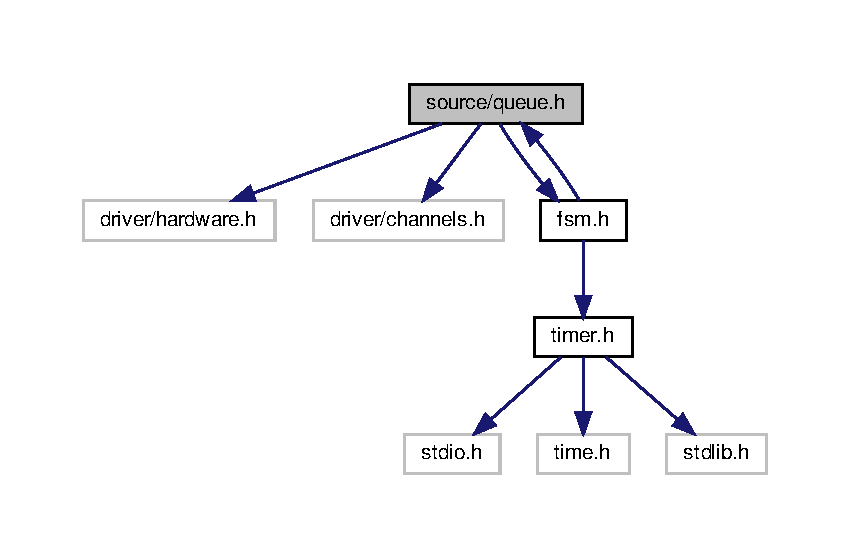
\includegraphics[width=350pt]{queue_8h__incl}
\end{center}
\end{figure}
This graph shows which files directly or indirectly include this file\+:
\nopagebreak
\begin{figure}[H]
\begin{center}
\leavevmode
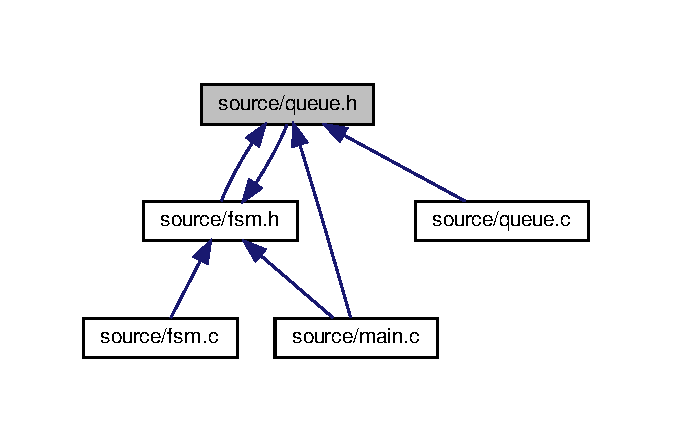
\includegraphics[width=323pt]{queue_8h__dep__incl}
\end{center}
\end{figure}
\subsection*{Enumerations}
\begin{DoxyCompactItemize}
\item 
\mbox{\Hypertarget{queue_8h_a3f7930823335655eba2f898c739671d0}\label{queue_8h_a3f7930823335655eba2f898c739671d0}} 
enum \hyperlink{queue_8h_a3f7930823335655eba2f898c739671d0}{elevator\+\_\+position} \{ \newline
{\bfseries first} = 0, 
{\bfseries second} = 1, 
{\bfseries third} = 2, 
{\bfseries fourth} = 3, 
\newline
{\bfseries first\+\_\+second} = 4, 
{\bfseries second\+\_\+third} = 5, 
{\bfseries third\+\_\+fourth} = 6
 \}\begin{DoxyCompactList}\small\item\em Enum containing the different positions of the elevator. \end{DoxyCompactList}
\end{DoxyCompactItemize}
\subsection*{Functions}
\begin{DoxyCompactItemize}
\item 
\mbox{\Hypertarget{queue_8h_a9d79c1ab7ae2f8d03fa045eae25f6b2a}\label{queue_8h_a9d79c1ab7ae2f8d03fa045eae25f6b2a}} 
void \hyperlink{queue_8h_a9d79c1ab7ae2f8d03fa045eae25f6b2a}{queue\+\_\+init\+\_\+queue} ()
\begin{DoxyCompactList}\small\item\em Initializes the queue matrix. \end{DoxyCompactList}\item 
int \hyperlink{queue_8h_af2004759a602f00d51d7a52b842ee27e}{queue\+\_\+queue\+\_\+exists} ()
\begin{DoxyCompactList}\small\item\em Checks if the queue contains order(s). \end{DoxyCompactList}\item 
\mbox{\Hypertarget{queue_8h_a3e5f178d15a689153f9d101a5e15b905}\label{queue_8h_a3e5f178d15a689153f9d101a5e15b905}} 
void \hyperlink{queue_8h_a3e5f178d15a689153f9d101a5e15b905}{queue\+\_\+iterate\+\_\+and\+\_\+update\+\_\+queue} ()
\begin{DoxyCompactList}\small\item\em Checks the hardware for orders and inserts them in the queue. Sets order-\/lights in hardware. \end{DoxyCompactList}\item 
int \hyperlink{queue_8h_a66cc5e1def51a8612fe8b6299c629ec3}{queue\+\_\+order\+\_\+above\+\_\+current\+\_\+position} (\hyperlink{queue_8h_a3f7930823335655eba2f898c739671d0}{elevator\+\_\+position} \hyperlink{queue_8h_a64aa88f4f8e0b2dc9d03a2177fb4241e}{position})
\begin{DoxyCompactList}\small\item\em Checks the queue for orders above the elevators current position. \end{DoxyCompactList}\item 
int \hyperlink{queue_8h_adec8b6fe8715213f3a8d98d6e7d2db14}{queue\+\_\+order\+\_\+below\+\_\+current\+\_\+position} (\hyperlink{queue_8h_a3f7930823335655eba2f898c739671d0}{elevator\+\_\+position} \hyperlink{queue_8h_a64aa88f4f8e0b2dc9d03a2177fb4241e}{position})
\begin{DoxyCompactList}\small\item\em Checks the queue for orders below the elevators current position. \end{DoxyCompactList}\item 
\mbox{\Hypertarget{queue_8h_a33400e4a7ea771bfe210a687747929ff}\label{queue_8h_a33400e4a7ea771bfe210a687747929ff}} 
void \hyperlink{queue_8h_a33400e4a7ea771bfe210a687747929ff}{queue\+\_\+delete\+\_\+queue} ()
\begin{DoxyCompactList}\small\item\em Removes all orders from queue. \end{DoxyCompactList}\item 
int \hyperlink{queue_8h_a5fcc64f8bb2774d86bfc8d7d1824d1ce}{queue\+\_\+order\+\_\+at\+\_\+floor\+\_\+number} (int floor)
\begin{DoxyCompactList}\small\item\em Checks if there exists orders at input floor. \end{DoxyCompactList}\item 
void \hyperlink{queue_8h_a62cd08b2aa5bdbff68e2c1d02e10f7a7}{queue\+\_\+remove\+\_\+order\+\_\+at\+\_\+floor\+\_\+number} (int floor)
\begin{DoxyCompactList}\small\item\em Removes all orders at the input floor from the queue. \end{DoxyCompactList}\item 
int \hyperlink{queue_8h_a3bc770d75f83b456f0e9a3137bbc6e77}{queue\+\_\+button\+\_\+inside\+\_\+at\+\_\+floor} (\hyperlink{queue_8h_a3f7930823335655eba2f898c739671d0}{elevator\+\_\+position} \hyperlink{queue_8h_a64aa88f4f8e0b2dc9d03a2177fb4241e}{position})
\begin{DoxyCompactList}\small\item\em Checks if the button inside of the elevator is pressed at the input position. \end{DoxyCompactList}\item 
int \hyperlink{queue_8h_af51d473de7a1809da941f124fa724dcf}{queue\+\_\+button\+\_\+down\+\_\+at\+\_\+floor} (\hyperlink{queue_8h_a3f7930823335655eba2f898c739671d0}{elevator\+\_\+position} \hyperlink{queue_8h_a64aa88f4f8e0b2dc9d03a2177fb4241e}{position})
\begin{DoxyCompactList}\small\item\em Checks if the down-\/button outside of the elevator is pressed at the input position. \end{DoxyCompactList}\item 
int \hyperlink{queue_8h_a14fc1d81de02daba4420f0b99bd3abbe}{queue\+\_\+button\+\_\+up\+\_\+at\+\_\+floor} (\hyperlink{queue_8h_a3f7930823335655eba2f898c739671d0}{elevator\+\_\+position} \hyperlink{queue_8h_a64aa88f4f8e0b2dc9d03a2177fb4241e}{position})
\begin{DoxyCompactList}\small\item\em Checks if the up-\/button outside of the elevator is pressed at the input position. \end{DoxyCompactList}\item 
\hyperlink{queue_8h_a3f7930823335655eba2f898c739671d0}{elevator\+\_\+position} \hyperlink{queue_8h_aa216eca86460fe50f3a10d176365813c}{queue\+\_\+get\+\_\+position} ()
\begin{DoxyCompactList}\small\item\em Get function for the elevators position. \end{DoxyCompactList}\item 
void \hyperlink{queue_8h_af44da6d1a5cb07cbe09f9b9886d24c2a}{queue\+\_\+set\+\_\+position} (\hyperlink{queue_8h_a3f7930823335655eba2f898c739671d0}{elevator\+\_\+position} pos)
\begin{DoxyCompactList}\small\item\em Set function for the elevators position. \end{DoxyCompactList}\end{DoxyCompactItemize}
\subsection*{Variables}
\begin{DoxyCompactItemize}
\item 
\mbox{\Hypertarget{queue_8h_a627865f7ba022b3ad9979791fc86a85f}\label{queue_8h_a627865f7ba022b3ad9979791fc86a85f}} 
int \hyperlink{queue_8h_a627865f7ba022b3ad9979791fc86a85f}{queue\+\_\+matrix} \mbox{[}H\+A\+R\+D\+W\+A\+R\+E\+\_\+\+N\+U\+M\+B\+E\+R\+\_\+\+O\+F\+\_\+\+F\+L\+O\+O\+RS\mbox{]}\mbox{[}H\+A\+R\+D\+W\+A\+R\+E\+\_\+\+N\+U\+M\+B\+E\+R\+\_\+\+O\+F\+\_\+\+B\+U\+T\+T\+O\+NS\mbox{]}
\begin{DoxyCompactList}\small\item\em 4x3 matrix containing all current orders in the system. \end{DoxyCompactList}\item 
\mbox{\Hypertarget{queue_8h_a64aa88f4f8e0b2dc9d03a2177fb4241e}\label{queue_8h_a64aa88f4f8e0b2dc9d03a2177fb4241e}} 
\hyperlink{queue_8h_a3f7930823335655eba2f898c739671d0}{elevator\+\_\+position} \hyperlink{queue_8h_a64aa88f4f8e0b2dc9d03a2177fb4241e}{position}
\begin{DoxyCompactList}\small\item\em Variable for storing the posistion of the elevator. \end{DoxyCompactList}\end{DoxyCompactItemize}


\subsection{Detailed Description}
.h-\/file for handling orders and managing the elevator queue. 



\subsection{Function Documentation}
\mbox{\Hypertarget{queue_8h_af51d473de7a1809da941f124fa724dcf}\label{queue_8h_af51d473de7a1809da941f124fa724dcf}} 
\index{queue.\+h@{queue.\+h}!queue\+\_\+button\+\_\+down\+\_\+at\+\_\+floor@{queue\+\_\+button\+\_\+down\+\_\+at\+\_\+floor}}
\index{queue\+\_\+button\+\_\+down\+\_\+at\+\_\+floor@{queue\+\_\+button\+\_\+down\+\_\+at\+\_\+floor}!queue.\+h@{queue.\+h}}
\subsubsection{\texorpdfstring{queue\+\_\+button\+\_\+down\+\_\+at\+\_\+floor()}{queue\_button\_down\_at\_floor()}}
{\footnotesize\ttfamily int queue\+\_\+button\+\_\+down\+\_\+at\+\_\+floor (\begin{DoxyParamCaption}\item[{\hyperlink{queue_8h_a3f7930823335655eba2f898c739671d0}{elevator\+\_\+position}}]{position }\end{DoxyParamCaption})}



Checks if the down-\/button outside of the elevator is pressed at the input position. 


\begin{DoxyParams}{Parameters}
{\em position} & Current position of the elevator. \\
\hline
\end{DoxyParams}
\begin{DoxyReturn}{Returns}
1 If the down-\/button outside of the elevator is pressed. 

0 If the down-\/button outside of the elevator is not pressed. 
\end{DoxyReturn}


Definition at line 108 of file queue.\+c.

\mbox{\Hypertarget{queue_8h_a3bc770d75f83b456f0e9a3137bbc6e77}\label{queue_8h_a3bc770d75f83b456f0e9a3137bbc6e77}} 
\index{queue.\+h@{queue.\+h}!queue\+\_\+button\+\_\+inside\+\_\+at\+\_\+floor@{queue\+\_\+button\+\_\+inside\+\_\+at\+\_\+floor}}
\index{queue\+\_\+button\+\_\+inside\+\_\+at\+\_\+floor@{queue\+\_\+button\+\_\+inside\+\_\+at\+\_\+floor}!queue.\+h@{queue.\+h}}
\subsubsection{\texorpdfstring{queue\+\_\+button\+\_\+inside\+\_\+at\+\_\+floor()}{queue\_button\_inside\_at\_floor()}}
{\footnotesize\ttfamily int queue\+\_\+button\+\_\+inside\+\_\+at\+\_\+floor (\begin{DoxyParamCaption}\item[{\hyperlink{queue_8h_a3f7930823335655eba2f898c739671d0}{elevator\+\_\+position}}]{position }\end{DoxyParamCaption})}



Checks if the button inside of the elevator is pressed at the input position. 


\begin{DoxyParams}{Parameters}
{\em position} & Current position of the elevator. \\
\hline
\end{DoxyParams}
\begin{DoxyReturn}{Returns}
1 If the inside-\/button i pressed. 

0 If the inside-\/button is not pressed. 
\end{DoxyReturn}


Definition at line 100 of file queue.\+c.

\mbox{\Hypertarget{queue_8h_a14fc1d81de02daba4420f0b99bd3abbe}\label{queue_8h_a14fc1d81de02daba4420f0b99bd3abbe}} 
\index{queue.\+h@{queue.\+h}!queue\+\_\+button\+\_\+up\+\_\+at\+\_\+floor@{queue\+\_\+button\+\_\+up\+\_\+at\+\_\+floor}}
\index{queue\+\_\+button\+\_\+up\+\_\+at\+\_\+floor@{queue\+\_\+button\+\_\+up\+\_\+at\+\_\+floor}!queue.\+h@{queue.\+h}}
\subsubsection{\texorpdfstring{queue\+\_\+button\+\_\+up\+\_\+at\+\_\+floor()}{queue\_button\_up\_at\_floor()}}
{\footnotesize\ttfamily int queue\+\_\+button\+\_\+up\+\_\+at\+\_\+floor (\begin{DoxyParamCaption}\item[{\hyperlink{queue_8h_a3f7930823335655eba2f898c739671d0}{elevator\+\_\+position}}]{position }\end{DoxyParamCaption})}



Checks if the up-\/button outside of the elevator is pressed at the input position. 


\begin{DoxyParams}{Parameters}
{\em position} & Current position of the elevator. \\
\hline
\end{DoxyParams}
\begin{DoxyReturn}{Returns}
1 If the up-\/button outside of the elevator is pressed. 

0 If the up-\/button outside of the elevator is not pressed. 
\end{DoxyReturn}


Definition at line 116 of file queue.\+c.

\mbox{\Hypertarget{queue_8h_aa216eca86460fe50f3a10d176365813c}\label{queue_8h_aa216eca86460fe50f3a10d176365813c}} 
\index{queue.\+h@{queue.\+h}!queue\+\_\+get\+\_\+position@{queue\+\_\+get\+\_\+position}}
\index{queue\+\_\+get\+\_\+position@{queue\+\_\+get\+\_\+position}!queue.\+h@{queue.\+h}}
\subsubsection{\texorpdfstring{queue\+\_\+get\+\_\+position()}{queue\_get\_position()}}
{\footnotesize\ttfamily \hyperlink{queue_8h_a3f7930823335655eba2f898c739671d0}{elevator\+\_\+position} queue\+\_\+get\+\_\+position (\begin{DoxyParamCaption}{ }\end{DoxyParamCaption})}



Get function for the elevators position. 

\begin{DoxyReturn}{Returns}
The current position of the elevator. 
\end{DoxyReturn}


Definition at line 124 of file queue.\+c.

\mbox{\Hypertarget{queue_8h_a66cc5e1def51a8612fe8b6299c629ec3}\label{queue_8h_a66cc5e1def51a8612fe8b6299c629ec3}} 
\index{queue.\+h@{queue.\+h}!queue\+\_\+order\+\_\+above\+\_\+current\+\_\+position@{queue\+\_\+order\+\_\+above\+\_\+current\+\_\+position}}
\index{queue\+\_\+order\+\_\+above\+\_\+current\+\_\+position@{queue\+\_\+order\+\_\+above\+\_\+current\+\_\+position}!queue.\+h@{queue.\+h}}
\subsubsection{\texorpdfstring{queue\+\_\+order\+\_\+above\+\_\+current\+\_\+position()}{queue\_order\_above\_current\_position()}}
{\footnotesize\ttfamily int queue\+\_\+order\+\_\+above\+\_\+current\+\_\+position (\begin{DoxyParamCaption}\item[{\hyperlink{queue_8h_a3f7930823335655eba2f898c739671d0}{elevator\+\_\+position}}]{position }\end{DoxyParamCaption})}



Checks the queue for orders above the elevators current position. 


\begin{DoxyParams}{Parameters}
{\em position} & Current position of the elevator. \\
\hline
\end{DoxyParams}
\begin{DoxyReturn}{Returns}
1 If there exists orders above current elevator position. 

0 If there are no orders above current elevator position. 
\end{DoxyReturn}


Definition at line 50 of file queue.\+c.

\mbox{\Hypertarget{queue_8h_a5fcc64f8bb2774d86bfc8d7d1824d1ce}\label{queue_8h_a5fcc64f8bb2774d86bfc8d7d1824d1ce}} 
\index{queue.\+h@{queue.\+h}!queue\+\_\+order\+\_\+at\+\_\+floor\+\_\+number@{queue\+\_\+order\+\_\+at\+\_\+floor\+\_\+number}}
\index{queue\+\_\+order\+\_\+at\+\_\+floor\+\_\+number@{queue\+\_\+order\+\_\+at\+\_\+floor\+\_\+number}!queue.\+h@{queue.\+h}}
\subsubsection{\texorpdfstring{queue\+\_\+order\+\_\+at\+\_\+floor\+\_\+number()}{queue\_order\_at\_floor\_number()}}
{\footnotesize\ttfamily int queue\+\_\+order\+\_\+at\+\_\+floor\+\_\+number (\begin{DoxyParamCaption}\item[{int}]{floor }\end{DoxyParamCaption})}



Checks if there exists orders at input floor. 


\begin{DoxyParams}{Parameters}
{\em floor} & Floor to check for orders. \\
\hline
\end{DoxyParams}
\begin{DoxyReturn}{Returns}
1 If there exists orders at input floor. 

0 If there are no orders at input floor. 
\end{DoxyReturn}


Definition at line 80 of file queue.\+c.

\mbox{\Hypertarget{queue_8h_adec8b6fe8715213f3a8d98d6e7d2db14}\label{queue_8h_adec8b6fe8715213f3a8d98d6e7d2db14}} 
\index{queue.\+h@{queue.\+h}!queue\+\_\+order\+\_\+below\+\_\+current\+\_\+position@{queue\+\_\+order\+\_\+below\+\_\+current\+\_\+position}}
\index{queue\+\_\+order\+\_\+below\+\_\+current\+\_\+position@{queue\+\_\+order\+\_\+below\+\_\+current\+\_\+position}!queue.\+h@{queue.\+h}}
\subsubsection{\texorpdfstring{queue\+\_\+order\+\_\+below\+\_\+current\+\_\+position()}{queue\_order\_below\_current\_position()}}
{\footnotesize\ttfamily int queue\+\_\+order\+\_\+below\+\_\+current\+\_\+position (\begin{DoxyParamCaption}\item[{\hyperlink{queue_8h_a3f7930823335655eba2f898c739671d0}{elevator\+\_\+position}}]{position }\end{DoxyParamCaption})}



Checks the queue for orders below the elevators current position. 


\begin{DoxyParams}{Parameters}
{\em position} & Current position of the elevator. \\
\hline
\end{DoxyParams}
\begin{DoxyReturn}{Returns}
1 If there exists orders below current elevator position. 

0 If there are no orders below current elevator position. 
\end{DoxyReturn}


Definition at line 60 of file queue.\+c.

\mbox{\Hypertarget{queue_8h_af2004759a602f00d51d7a52b842ee27e}\label{queue_8h_af2004759a602f00d51d7a52b842ee27e}} 
\index{queue.\+h@{queue.\+h}!queue\+\_\+queue\+\_\+exists@{queue\+\_\+queue\+\_\+exists}}
\index{queue\+\_\+queue\+\_\+exists@{queue\+\_\+queue\+\_\+exists}!queue.\+h@{queue.\+h}}
\subsubsection{\texorpdfstring{queue\+\_\+queue\+\_\+exists()}{queue\_queue\_exists()}}
{\footnotesize\ttfamily int queue\+\_\+queue\+\_\+exists (\begin{DoxyParamCaption}{ }\end{DoxyParamCaption})}



Checks if the queue contains order(s). 

\begin{DoxyReturn}{Returns}
1 If order(s) in queue. 

0 If no orders in queue. 
\end{DoxyReturn}


Definition at line 24 of file queue.\+c.

\mbox{\Hypertarget{queue_8h_a62cd08b2aa5bdbff68e2c1d02e10f7a7}\label{queue_8h_a62cd08b2aa5bdbff68e2c1d02e10f7a7}} 
\index{queue.\+h@{queue.\+h}!queue\+\_\+remove\+\_\+order\+\_\+at\+\_\+floor\+\_\+number@{queue\+\_\+remove\+\_\+order\+\_\+at\+\_\+floor\+\_\+number}}
\index{queue\+\_\+remove\+\_\+order\+\_\+at\+\_\+floor\+\_\+number@{queue\+\_\+remove\+\_\+order\+\_\+at\+\_\+floor\+\_\+number}!queue.\+h@{queue.\+h}}
\subsubsection{\texorpdfstring{queue\+\_\+remove\+\_\+order\+\_\+at\+\_\+floor\+\_\+number()}{queue\_remove\_order\_at\_floor\_number()}}
{\footnotesize\ttfamily void queue\+\_\+remove\+\_\+order\+\_\+at\+\_\+floor\+\_\+number (\begin{DoxyParamCaption}\item[{int}]{floor }\end{DoxyParamCaption})}



Removes all orders at the input floor from the queue. 


\begin{DoxyParams}{Parameters}
{\em floor} & The floor which should be cleared for orders in the queue. \\
\hline
\end{DoxyParams}


Definition at line 90 of file queue.\+c.

\mbox{\Hypertarget{queue_8h_af44da6d1a5cb07cbe09f9b9886d24c2a}\label{queue_8h_af44da6d1a5cb07cbe09f9b9886d24c2a}} 
\index{queue.\+h@{queue.\+h}!queue\+\_\+set\+\_\+position@{queue\+\_\+set\+\_\+position}}
\index{queue\+\_\+set\+\_\+position@{queue\+\_\+set\+\_\+position}!queue.\+h@{queue.\+h}}
\subsubsection{\texorpdfstring{queue\+\_\+set\+\_\+position()}{queue\_set\_position()}}
{\footnotesize\ttfamily void queue\+\_\+set\+\_\+position (\begin{DoxyParamCaption}\item[{\hyperlink{queue_8h_a3f7930823335655eba2f898c739671d0}{elevator\+\_\+position}}]{pos }\end{DoxyParamCaption})}



Set function for the elevators position. 


\begin{DoxyParams}{Parameters}
{\em pos} & The position elevator position is changed to. \\
\hline
\end{DoxyParams}


Definition at line 129 of file queue.\+c.


\hypertarget{timer_8c}{}\section{source/timer.c File Reference}
\label{timer_8c}\index{source/timer.\+c@{source/timer.\+c}}


.c-\/file for the timer system.  


{\ttfamily \#include \char`\"{}timer.\+h\char`\"{}}\newline
{\ttfamily \#include $<$time.\+h$>$}\newline
Include dependency graph for timer.\+c\+:
\nopagebreak
\begin{figure}[H]
\begin{center}
\leavevmode
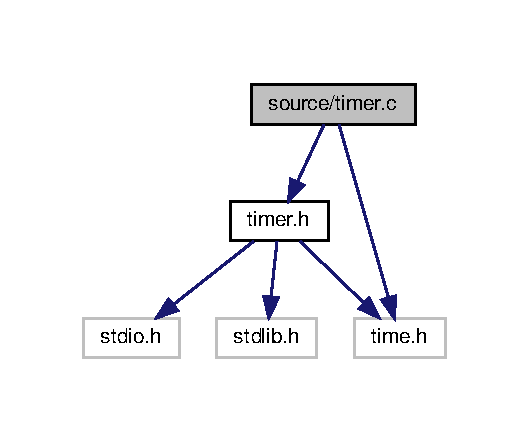
\includegraphics[width=254pt]{timer_8c__incl}
\end{center}
\end{figure}
\subsection*{Functions}
\begin{DoxyCompactItemize}
\item 
\mbox{\Hypertarget{timer_8c_a232289df78f39fca1fdfc992176a5d75}\label{timer_8c_a232289df78f39fca1fdfc992176a5d75}} 
void \hyperlink{timer_8c_a232289df78f39fca1fdfc992176a5d75}{timer\+\_\+start\+\_\+timer} ()
\begin{DoxyCompactList}\small\item\em Starts a timer. \end{DoxyCompactList}\item 
int \hyperlink{timer_8c_a68e0e1d10f743a641770ac85ec5abe99}{timer\+\_\+timer\+\_\+has\+\_\+expried} (double seconds)
\begin{DoxyCompactList}\small\item\em Checks for how long the timer\+\_\+counter variable has been running for. \end{DoxyCompactList}\end{DoxyCompactItemize}


\subsection{Detailed Description}
.c-\/file for the timer system. 



\subsection{Function Documentation}
\mbox{\Hypertarget{timer_8c_a68e0e1d10f743a641770ac85ec5abe99}\label{timer_8c_a68e0e1d10f743a641770ac85ec5abe99}} 
\index{timer.\+c@{timer.\+c}!timer\+\_\+timer\+\_\+has\+\_\+expried@{timer\+\_\+timer\+\_\+has\+\_\+expried}}
\index{timer\+\_\+timer\+\_\+has\+\_\+expried@{timer\+\_\+timer\+\_\+has\+\_\+expried}!timer.\+c@{timer.\+c}}
\subsubsection{\texorpdfstring{timer\+\_\+timer\+\_\+has\+\_\+expried()}{timer\_timer\_has\_expried()}}
{\footnotesize\ttfamily int timer\+\_\+timer\+\_\+has\+\_\+expried (\begin{DoxyParamCaption}\item[{double}]{seconds }\end{DoxyParamCaption})}



Checks for how long the timer\+\_\+counter variable has been running for. 


\begin{DoxyParams}{Parameters}
{\em seconds} & The time you want to let go by before the function returns True. \\
\hline
\end{DoxyParams}
\begin{DoxyReturn}{Returns}
1 if it has gone by more than or equal to seconds seconds since the timer started in \hyperlink{timer_8h_a232289df78f39fca1fdfc992176a5d75}{timer\+\_\+start\+\_\+timer()}. 

0 if it has gone by less than seconds seconds since the timer started in \hyperlink{timer_8h_a232289df78f39fca1fdfc992176a5d75}{timer\+\_\+start\+\_\+timer()}. 
\end{DoxyReturn}


Definition at line 19 of file timer.\+c.


\hypertarget{timer_8h}{}\section{source/timer.h File Reference}
\label{timer_8h}\index{source/timer.\+h@{source/timer.\+h}}


.h-\/file for the timer system.  


{\ttfamily \#include $<$stdio.\+h$>$}\newline
{\ttfamily \#include $<$time.\+h$>$}\newline
{\ttfamily \#include $<$stdlib.\+h$>$}\newline
Include dependency graph for timer.\+h\+:
\nopagebreak
\begin{figure}[H]
\begin{center}
\leavevmode
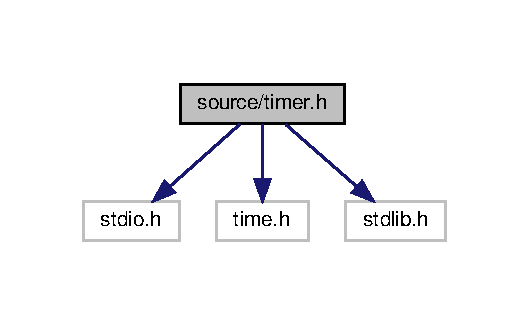
\includegraphics[width=254pt]{timer_8h__incl}
\end{center}
\end{figure}
This graph shows which files directly or indirectly include this file\+:
\nopagebreak
\begin{figure}[H]
\begin{center}
\leavevmode
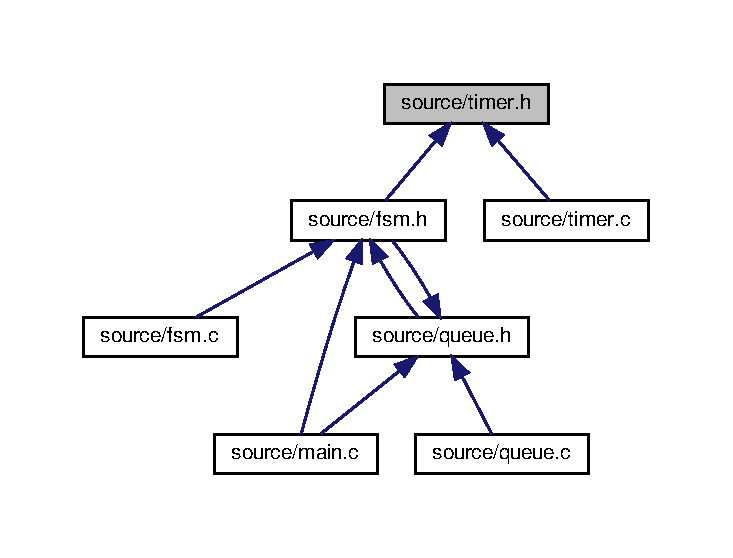
\includegraphics[width=350pt]{timer_8h__dep__incl}
\end{center}
\end{figure}
\subsection*{Functions}
\begin{DoxyCompactItemize}
\item 
\mbox{\Hypertarget{timer_8h_a232289df78f39fca1fdfc992176a5d75}\label{timer_8h_a232289df78f39fca1fdfc992176a5d75}} 
void \hyperlink{timer_8h_a232289df78f39fca1fdfc992176a5d75}{timer\+\_\+start\+\_\+timer} ()
\begin{DoxyCompactList}\small\item\em Starts a timer. \end{DoxyCompactList}\item 
int \hyperlink{timer_8h_a68e0e1d10f743a641770ac85ec5abe99}{timer\+\_\+timer\+\_\+has\+\_\+expried} (double seconds)
\begin{DoxyCompactList}\small\item\em Checks for how long the timer\+\_\+counter variable has been running for. \end{DoxyCompactList}\end{DoxyCompactItemize}


\subsection{Detailed Description}
.h-\/file for the timer system. 



\subsection{Function Documentation}
\mbox{\Hypertarget{timer_8h_a68e0e1d10f743a641770ac85ec5abe99}\label{timer_8h_a68e0e1d10f743a641770ac85ec5abe99}} 
\index{timer.\+h@{timer.\+h}!timer\+\_\+timer\+\_\+has\+\_\+expried@{timer\+\_\+timer\+\_\+has\+\_\+expried}}
\index{timer\+\_\+timer\+\_\+has\+\_\+expried@{timer\+\_\+timer\+\_\+has\+\_\+expried}!timer.\+h@{timer.\+h}}
\subsubsection{\texorpdfstring{timer\+\_\+timer\+\_\+has\+\_\+expried()}{timer\_timer\_has\_expried()}}
{\footnotesize\ttfamily int timer\+\_\+timer\+\_\+has\+\_\+expried (\begin{DoxyParamCaption}\item[{double}]{seconds }\end{DoxyParamCaption})}



Checks for how long the timer\+\_\+counter variable has been running for. 


\begin{DoxyParams}{Parameters}
{\em seconds} & The time you want to let go by before the function returns True. \\
\hline
\end{DoxyParams}
\begin{DoxyReturn}{Returns}
1 if it has gone by more than or equal to seconds seconds since the timer started in \hyperlink{timer_8h_a232289df78f39fca1fdfc992176a5d75}{timer\+\_\+start\+\_\+timer()}. 

0 if it has gone by less than seconds seconds since the timer started in \hyperlink{timer_8h_a232289df78f39fca1fdfc992176a5d75}{timer\+\_\+start\+\_\+timer()}. 
\end{DoxyReturn}


Definition at line 19 of file timer.\+c.


%--- End generated contents ---

% Index
\backmatter
\newpage
\phantomsection
\clearemptydoublepage
\addcontentsline{toc}{chapter}{Index}
\printindex

\end{document}
